\documentclass{article}
\usepackage{graphicx}
\usepackage[utf8]{inputenc}
\usepackage[T1]{fontenc}
\usepackage{lmodern}
\usepackage{float}
\usepackage{caption}
\usepackage{subcaption}
\usepackage[paperwidth=4.1in, paperheight=5.8in, margin=0.25in]{geometry}
\renewcommand*\familydefault{\sfdefault}
\pagenumbering{gobble}

\usepackage{pgfmorepages}

\pgfpagesdeclarelayout{8 on 2, book format}
{%
  \edef\pgfpageoptionheight{\the\paperheight}
  \edef\pgfpageoptionwidth{\the\paperwidth}
  \def\pgfpageoptionborder{0pt}
  \def\pgfpageoptionfirstshipout{1}
}%
{%
  \pgfpagesphysicalpageoptions
  {%
    logical pages=8,%
    physical pages=2,%
    physical height=\pgfpageoptionheight,%
    physical width=\pgfpageoptionwidth,%
    current logical shipout=\pgfpageoptionfirstshipout%
  }
  \pgfpagesphysicalpage{1}{}
    \pgfpageslogicalpageoptions{4}
    {%
      border shrink=\pgfpageoptionborder,%
      resized width=.5\pgfphysicalwidth,%
      resized height=.5\pgfphysicalheight,%
      center=\pgfpoint{.25\pgfphysicalwidth}{.75\pgfphysicalheight}%
    }%
    \pgfpageslogicalpageoptions{2}
    {%
      border shrink=\pgfpageoptionborder,%
      resized width=.5\pgfphysicalwidth,%
      resized height=.5\pgfphysicalheight,%
      center=\pgfpoint{.75\pgfphysicalwidth}{.75\pgfphysicalheight}%
    }%
    \pgfpageslogicalpageoptions{8}
    {%
      border shrink=\pgfpageoptionborder,%
      resized width=.5\pgfphysicalwidth,%
      resized height=.5\pgfphysicalheight,%
      center=\pgfpoint{.25\pgfphysicalwidth}{.25\pgfphysicalheight},%
    }%
    \pgfpageslogicalpageoptions{6}
    {%
      border shrink=\pgfpageoptionborder,%
      resized width=.5\pgfphysicalwidth,%
      resized height=.5\pgfphysicalheight,%
      center=\pgfpoint{.75\pgfphysicalwidth}{.25\pgfphysicalheight},%
    }%
  \pgfpagesphysicalpage{2}{}
    \pgfpageslogicalpageoptions{1}
    {%
      border shrink=\pgfpageoptionborder,%
      resized width=.5\pgfphysicalwidth,%
      resized height=.5\pgfphysicalheight,%
      center=\pgfpoint{.25\pgfphysicalwidth}{.75\pgfphysicalheight}%
    }%
    \pgfpageslogicalpageoptions{3}
    {%
      border shrink=\pgfpageoptionborder,%
      resized width=.5\pgfphysicalwidth,%
      resized height=.5\pgfphysicalheight,%
      center=\pgfpoint{.75\pgfphysicalwidth}{.75\pgfphysicalheight}%
    }%
    \pgfpageslogicalpageoptions{5}
    {%
      border shrink=\pgfpageoptionborder,%
      resized width=.5\pgfphysicalwidth,%
      resized height=.5\pgfphysicalheight,%
      center=\pgfpoint{.25\pgfphysicalwidth}{.25\pgfphysicalheight},%
    }%
    \pgfpageslogicalpageoptions{7}
    {%
      border shrink=\pgfpageoptionborder,%
      resized width=.5\pgfphysicalwidth,%
      resized height=.5\pgfphysicalheight,%
      center=\pgfpoint{.75\pgfphysicalwidth}{.25\pgfphysicalheight},%
    }%
}


\pgfpagesuselayout{8 on 2, book format}[a4paper]
\begin{document}
    
        \par\noindent\rule{\textwidth}{0.4pt}
    \begin{figure}[H]
        \centering
        \begin{minipage}{0.25\textwidth}
            \centering
            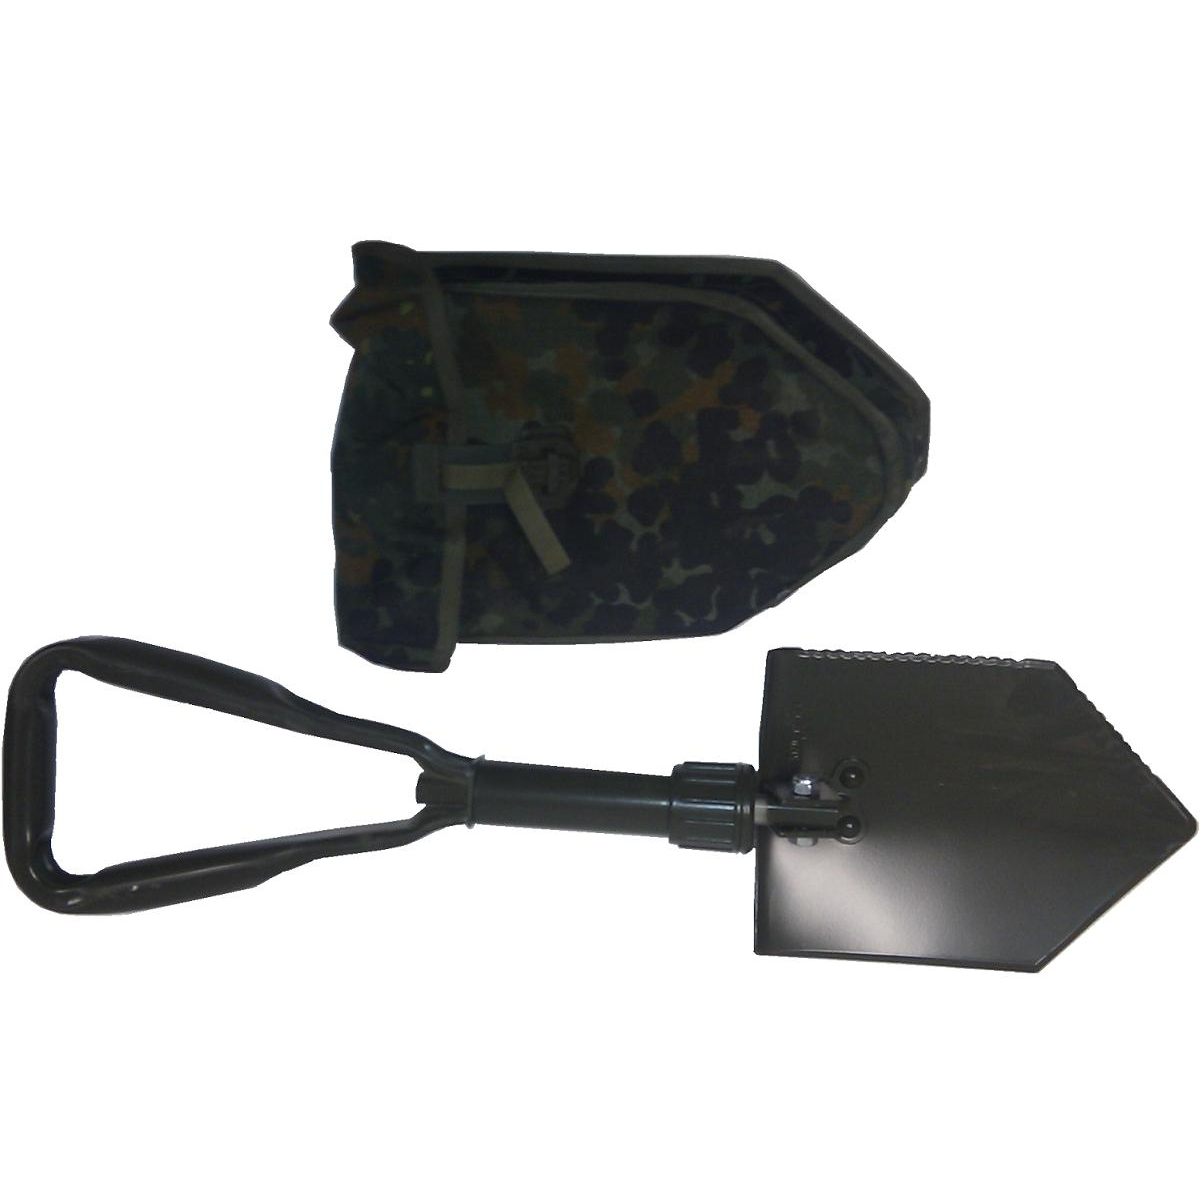
\includegraphics[width=\textwidth]{../SurvivalItemImages/foldingshovel}
        \end{minipage}\hfill
        \begin{minipage}{0.7\textwidth}
            \centering
            \Large Folding shovel
        \end{minipage}
    \end{figure}
    \vspace{-0.8em}
    \noindent\rule{\textwidth}{0.4pt}
            
    \begin{figure}[H]
        \centering
        \begin{minipage}{0.25\textwidth}
            \centering
            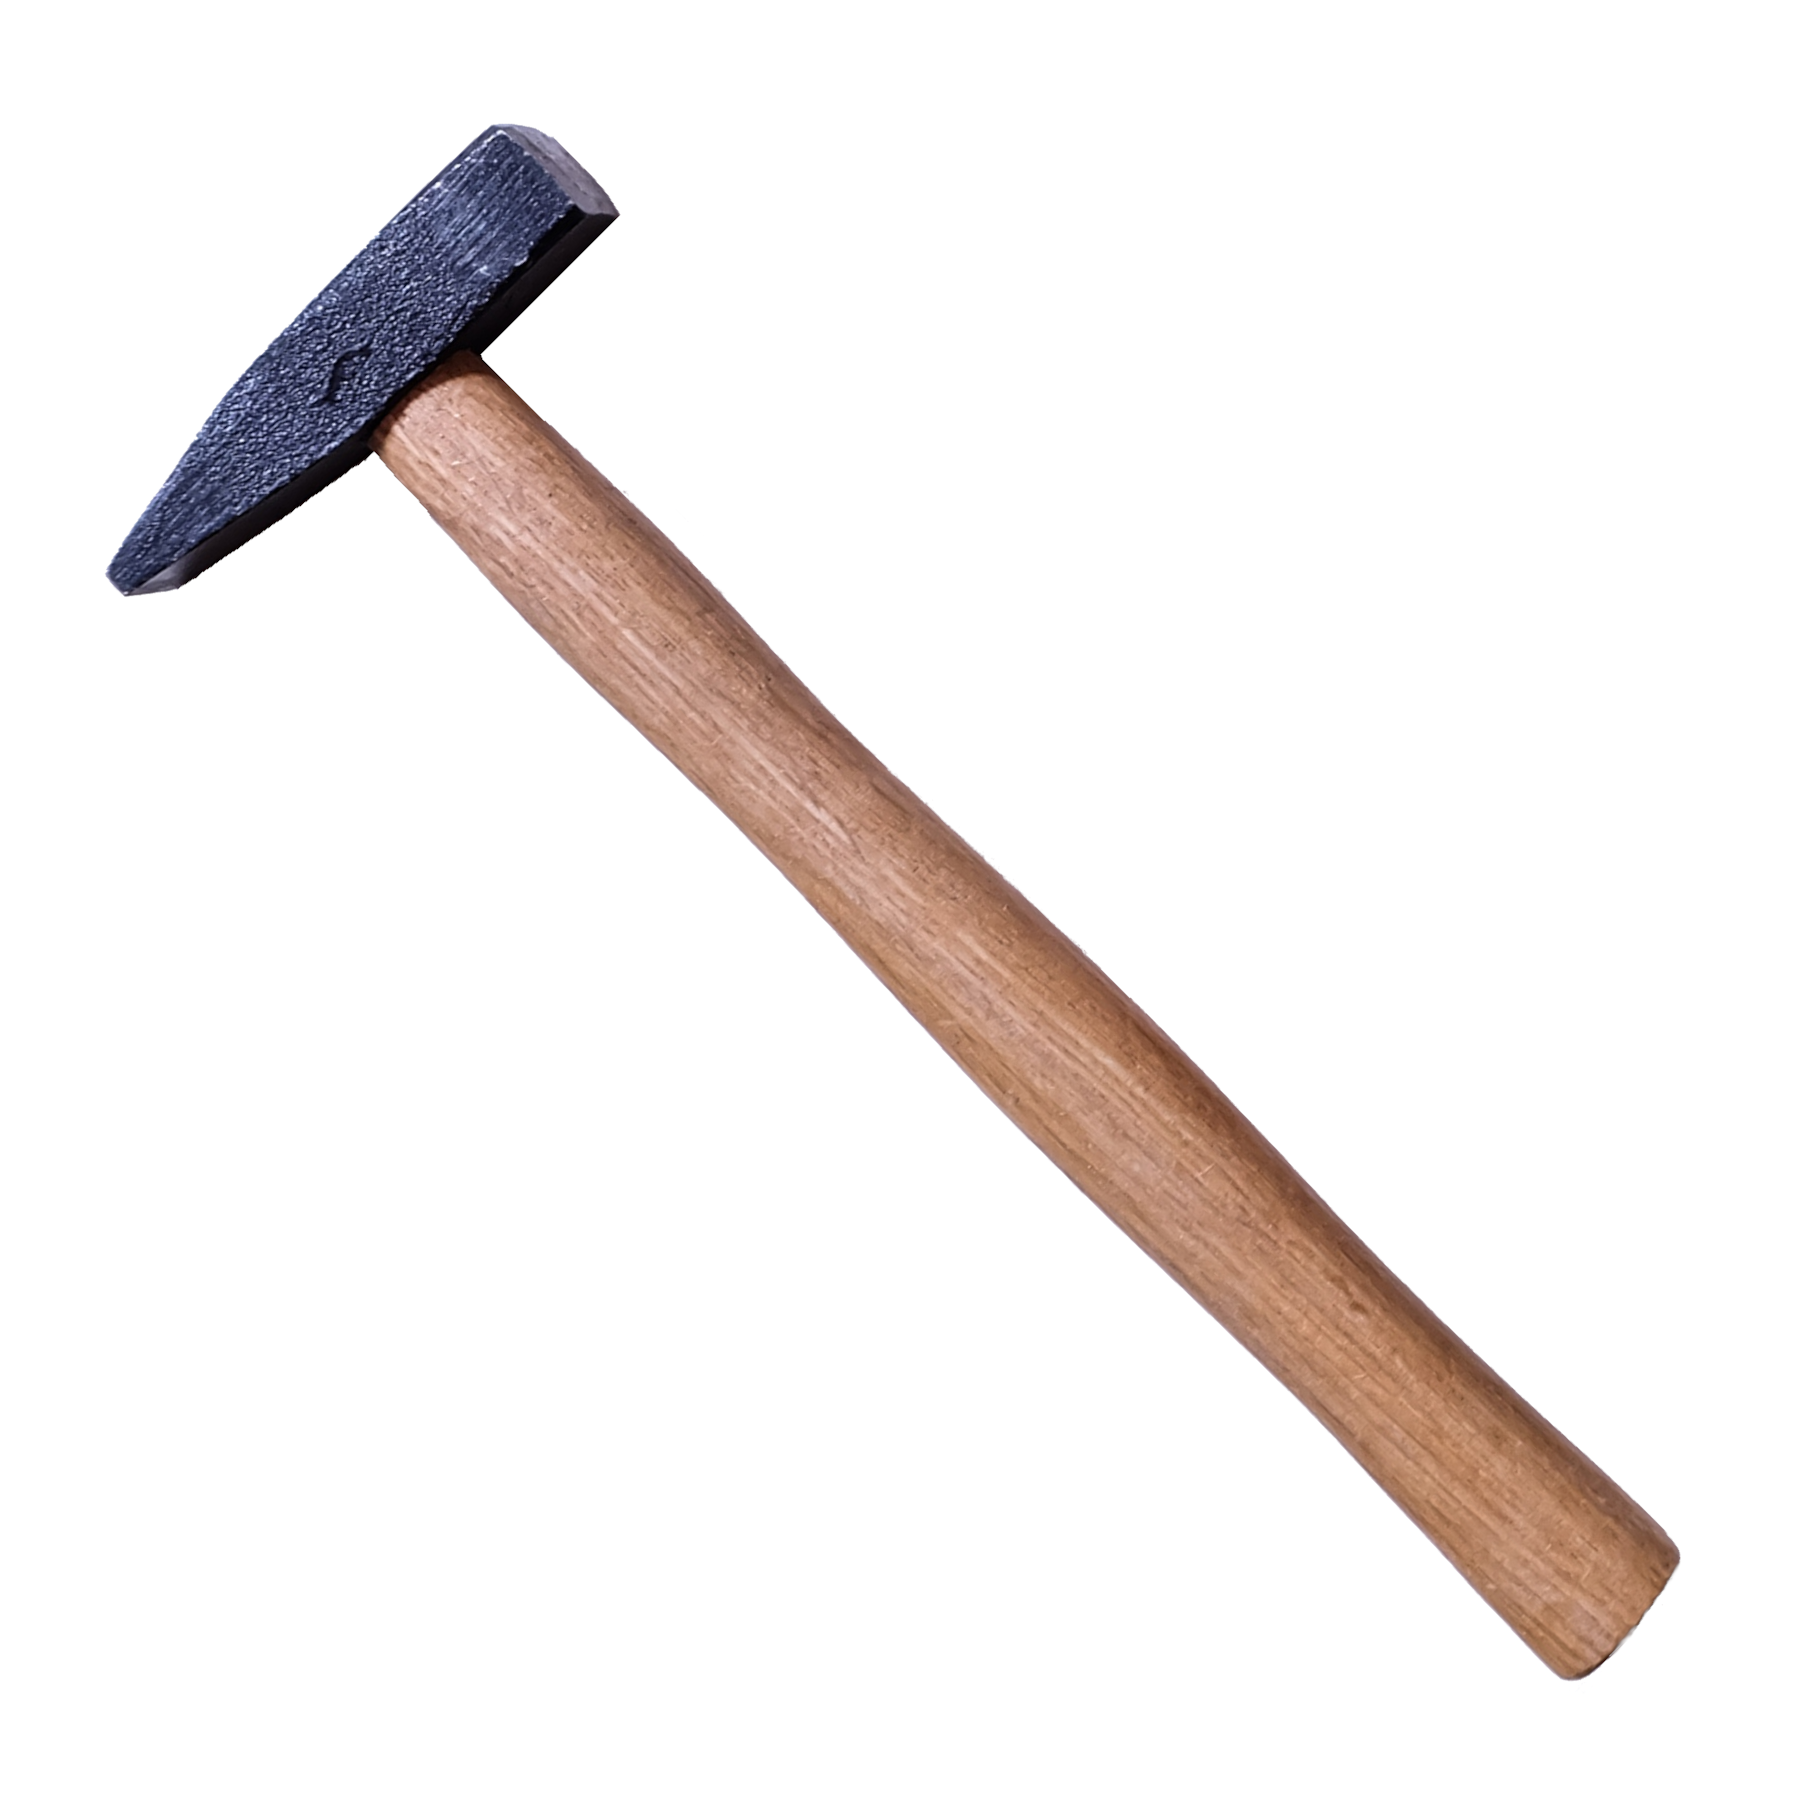
\includegraphics[width=\textwidth]{../SurvivalItemImages/hammer}
        \end{minipage}\hfill
        \begin{minipage}{0.7\textwidth}
            \centering
            \Large Hammer
        \end{minipage}
    \end{figure}
    \vspace{-0.8em}
    \noindent\rule{\textwidth}{0.4pt}
            
    \begin{figure}[H]
        \centering
        \begin{minipage}{0.25\textwidth}
            \centering
            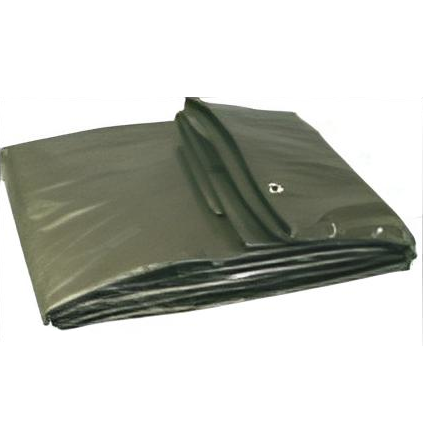
\includegraphics[width=\textwidth]{../SurvivalItemImages/plasticsheeting}
        \end{minipage}\hfill
        \begin{minipage}{0.7\textwidth}
            \centering
            \Large 20 square feet of opaque plastic sheeting
        \end{minipage}
    \end{figure}
    \vspace{-0.8em}
    \noindent\rule{\textwidth}{0.4pt}
            
    \begin{figure}[H]
        \centering
        \begin{minipage}{0.25\textwidth}
            \centering
            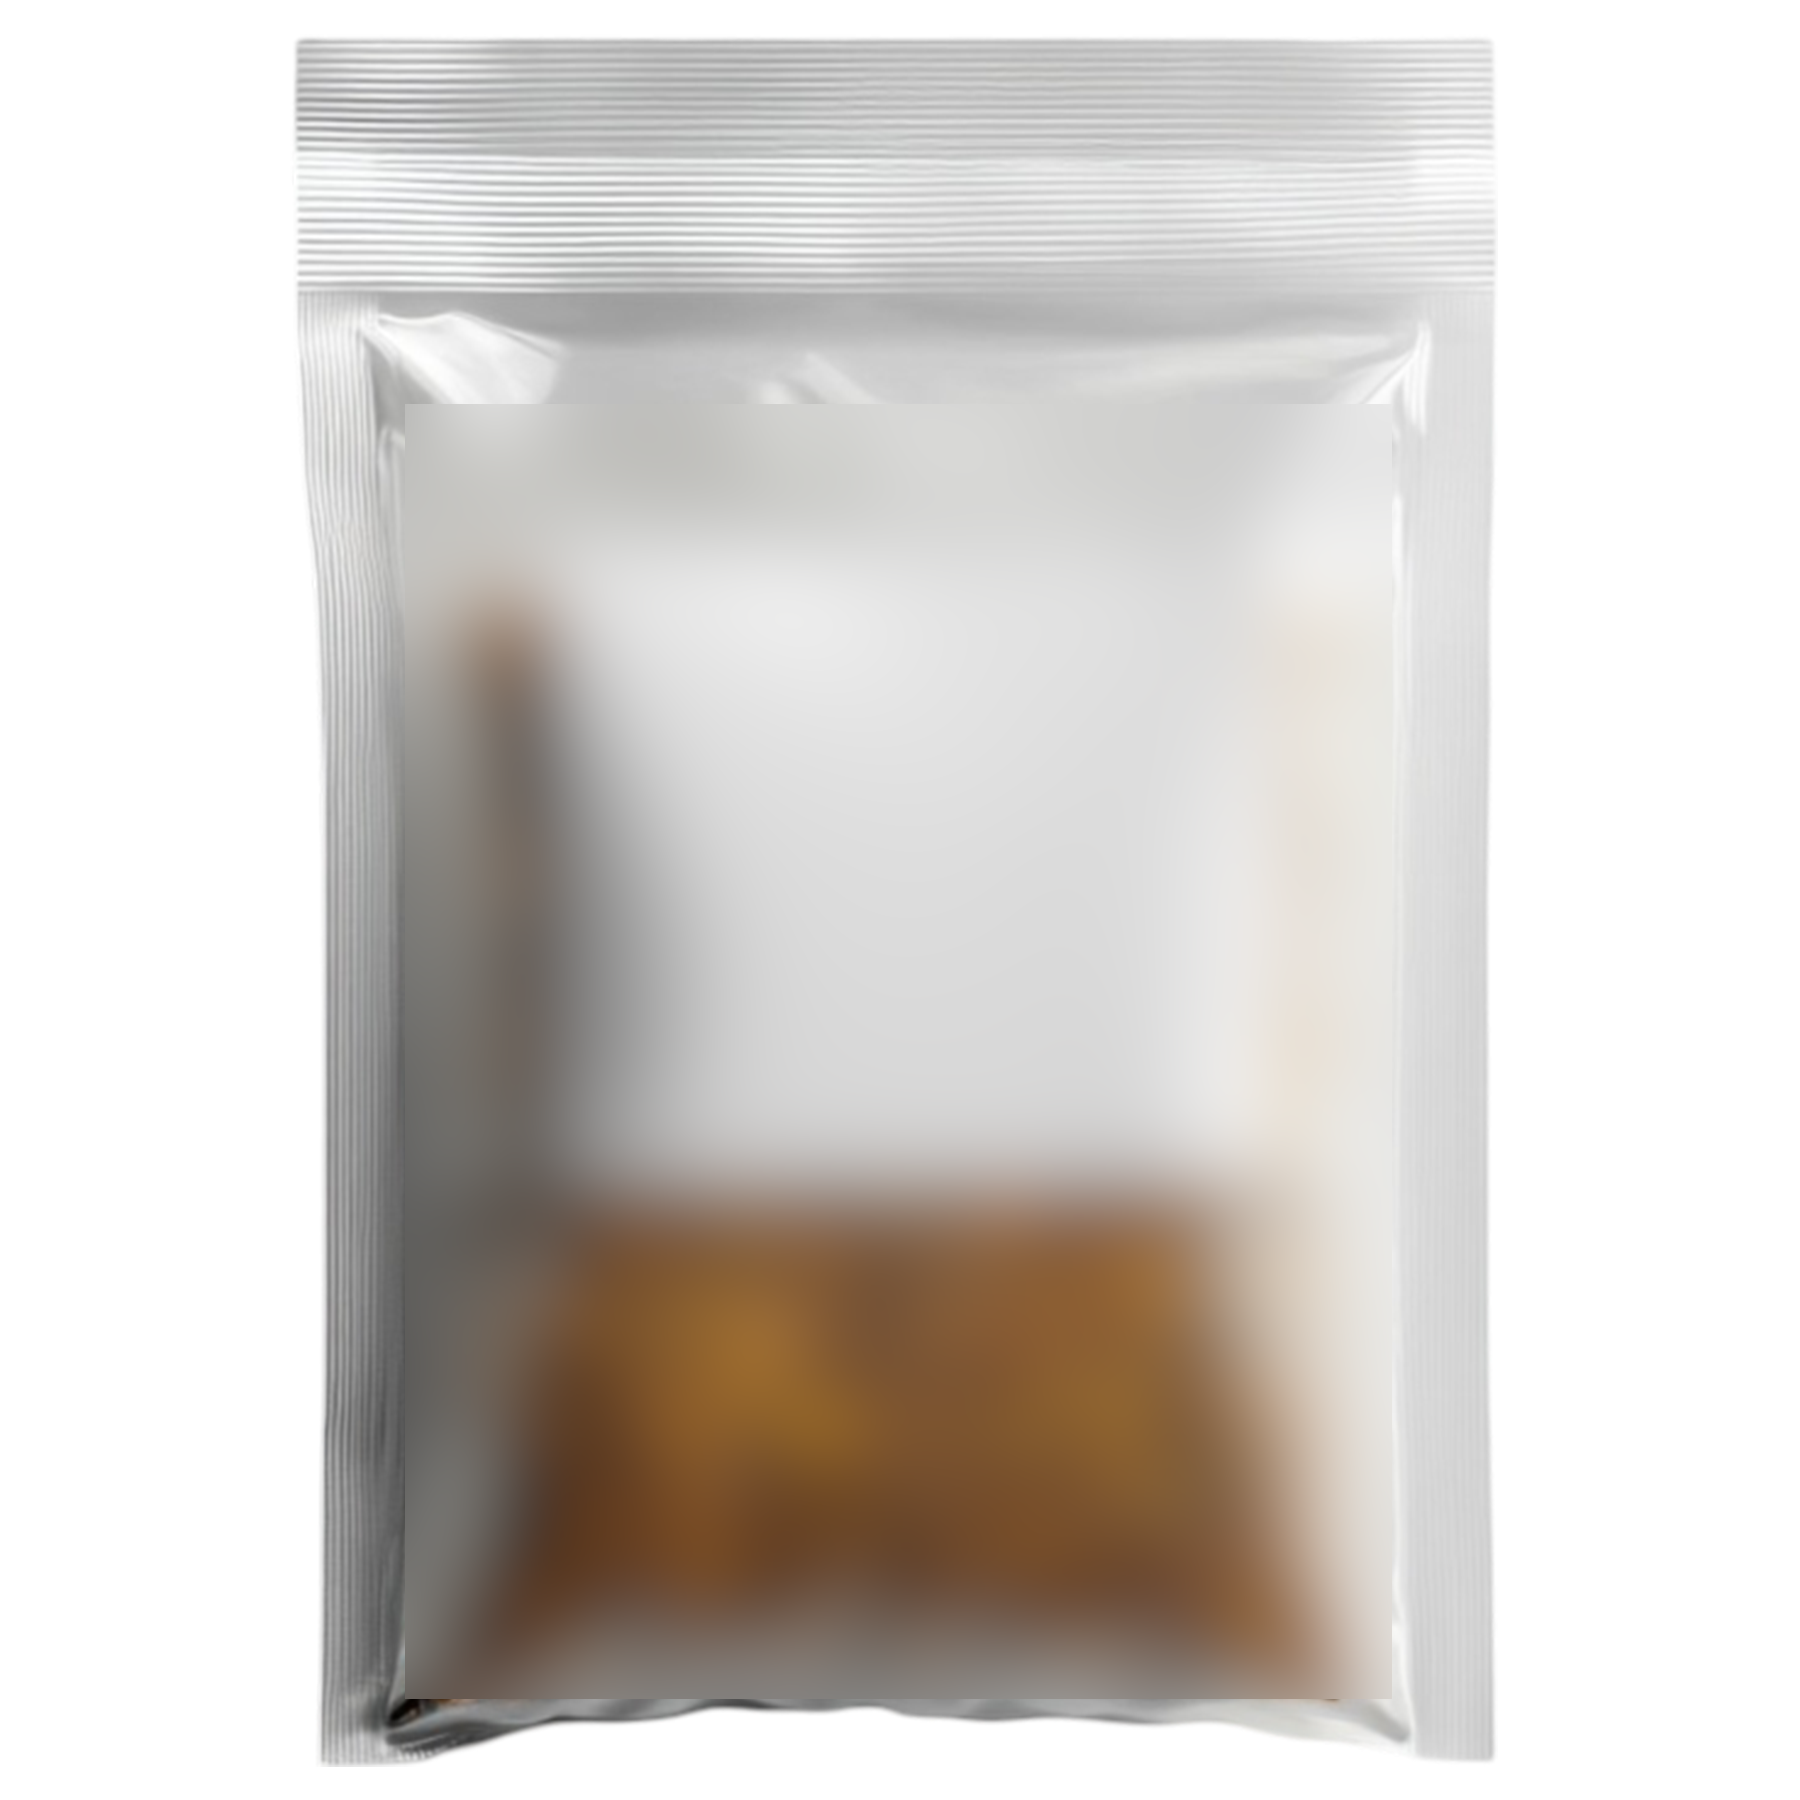
\includegraphics[width=\textwidth]{../SurvivalItemImages/concentrate}
        \end{minipage}\hfill
        \begin{minipage}{0.7\textwidth}
            \centering
            \Large Food concentrate
        \end{minipage}
    \end{figure}
    \vspace{-0.8em}
    \noindent\rule{\textwidth}{0.4pt}
            
    \clearpage
    \section*{Scenario: \textmd{Cavelabyrinth} \hfill Participant \textmd{0}}
    \Large You were on a tour through a large cave labyrinth with underground lakes for several days now. A tunnel crashed down, you and two fellow travelers were separated from the tour guide and the rest of the group. You also lost all possibilities to contact the others. Fortunately no one is injured and your protective clothes and helmet lamps are in good condition. The evening before, the tour guide explained that there are several exits from the cave, but it takes several days to reach those and one needs to cross some of the underground lakes. On your side of the collapsed tunnel you could find some items.\clearpage
        \par\noindent\rule{\textwidth}{0.4pt}
    \begin{figure}[H]
        \centering
        \begin{minipage}{0.25\textwidth}
            \centering
            \includegraphics[width=\textwidth]{../SurvivalItemImages/rubberboat}
        \end{minipage}\hfill
        \begin{minipage}{0.7\textwidth}
            \centering
            \Large Portable rubber boat
        \end{minipage}
    \end{figure}
    \vspace{-0.8em}
    \noindent\rule{\textwidth}{0.4pt}
            
    \begin{figure}[H]
        \centering
        \begin{minipage}{0.25\textwidth}
            \centering
            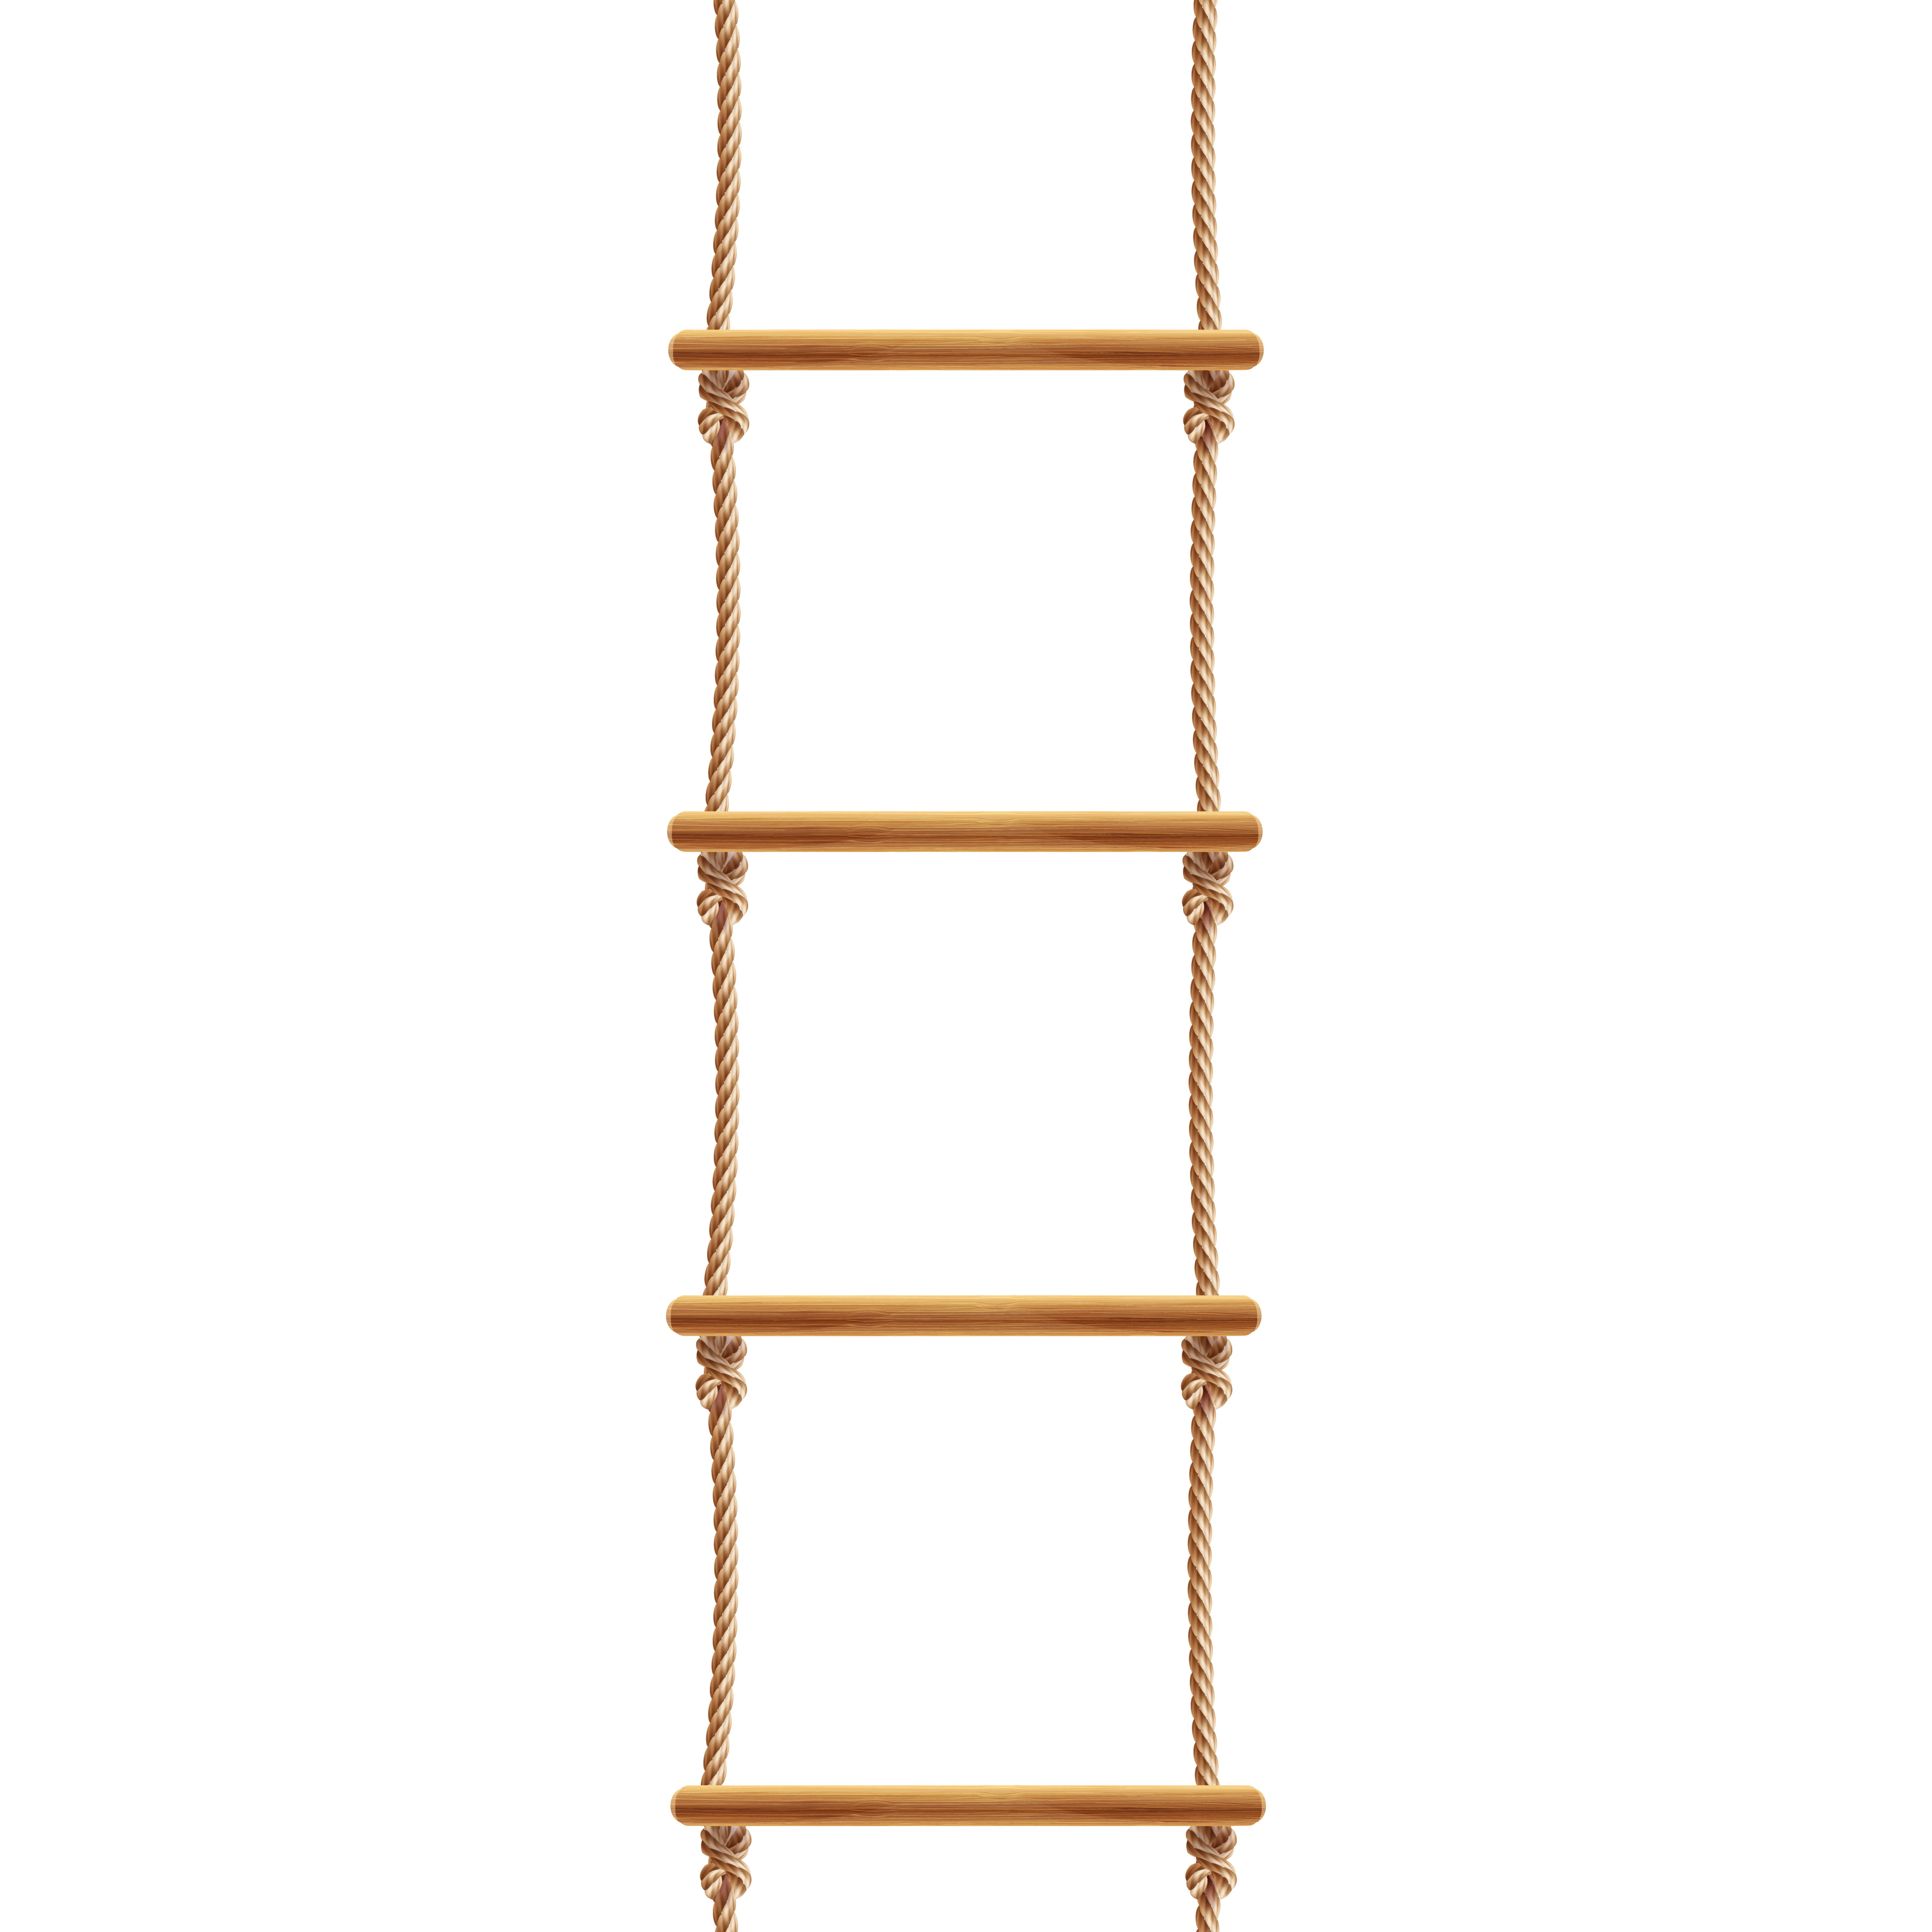
\includegraphics[width=\textwidth]{../SurvivalItemImages/ropeladder}
        \end{minipage}\hfill
        \begin{minipage}{0.7\textwidth}
            \centering
            \Large Rope ladder
        \end{minipage}
    \end{figure}
    \vspace{-0.8em}
    \noindent\rule{\textwidth}{0.4pt}
            
    \begin{figure}[H]
        \centering
        \begin{minipage}{0.25\textwidth}
            \centering
            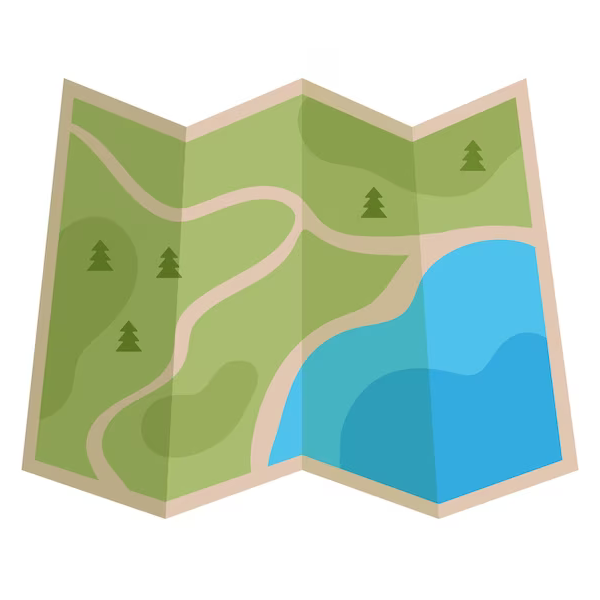
\includegraphics[width=\textwidth]{../SurvivalItemImages/map}
        \end{minipage}\hfill
        \begin{minipage}{0.7\textwidth}
            \centering
            \Large A map of the cave labyrinth
        \end{minipage}
    \end{figure}
    \vspace{-0.8em}
    \noindent\rule{\textwidth}{0.4pt}
            
    \begin{figure}[H]
        \centering
        \begin{minipage}{0.25\textwidth}
            \centering
            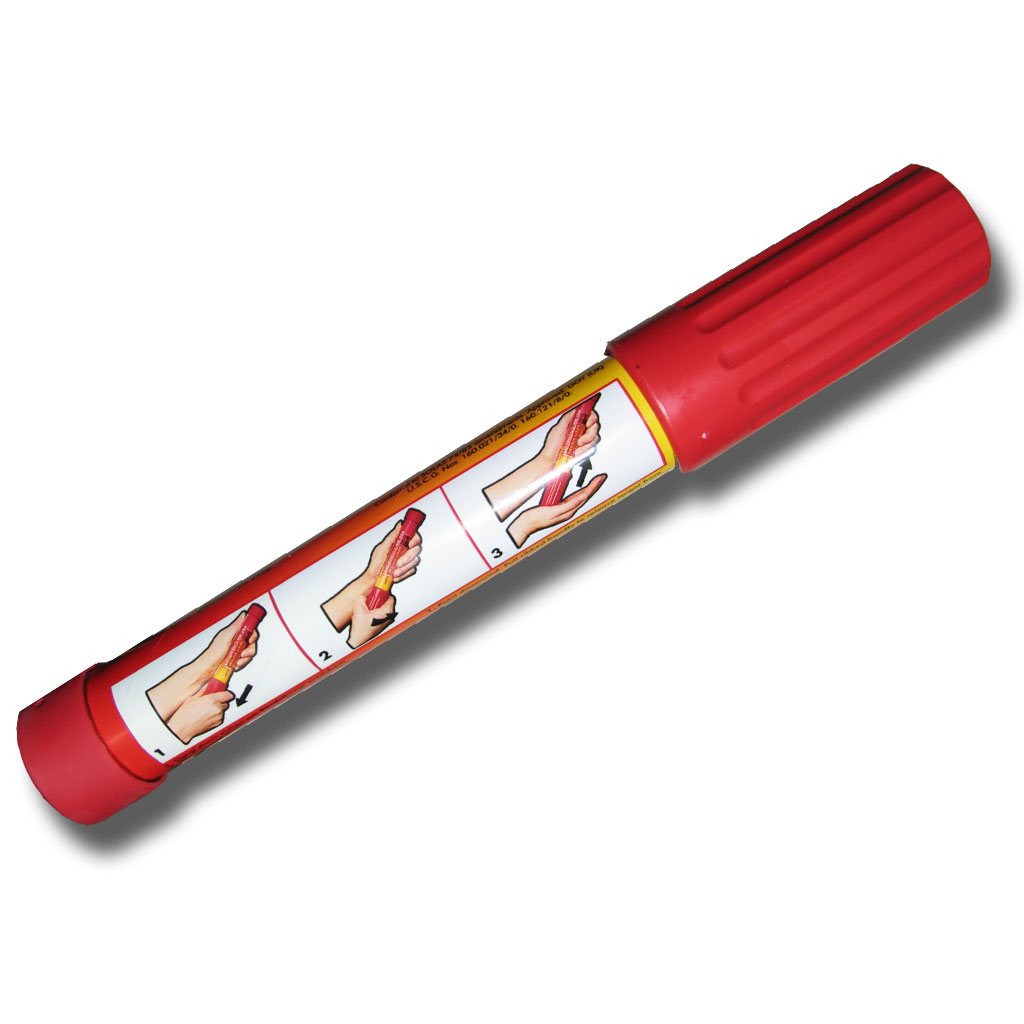
\includegraphics[width=\textwidth]{../SurvivalItemImages/flares}
        \end{minipage}\hfill
        \begin{minipage}{0.7\textwidth}
            \centering
            \Large Three signal flares
        \end{minipage}
    \end{figure}
    \vspace{-0.8em}
    \noindent\rule{\textwidth}{0.4pt}
            
    \clearpage
    \section*{Scenario: \textmd{Cavelabyrinth} \hfill Participant \textmd{1}}
    \Large You were on a tour through a large cave labyrinth with underground lakes for several days now. A tunnel crashed down, you and two fellow travelers were separated from the tour guide and the rest of the group. You also lost all possibilities to contact the others. Fortunately no one is injured and your protective clothes and helmet lamps are in good condition. The evening before, the tour guide explained that there are several exits from the cave, but it takes several days to reach those and one needs to cross some of the underground lakes. On your side of the collapsed tunnel you could find some items.\clearpage
        \par\noindent\rule{\textwidth}{0.4pt}
    \begin{figure}[H]
        \centering
        \begin{minipage}{0.25\textwidth}
            \centering
            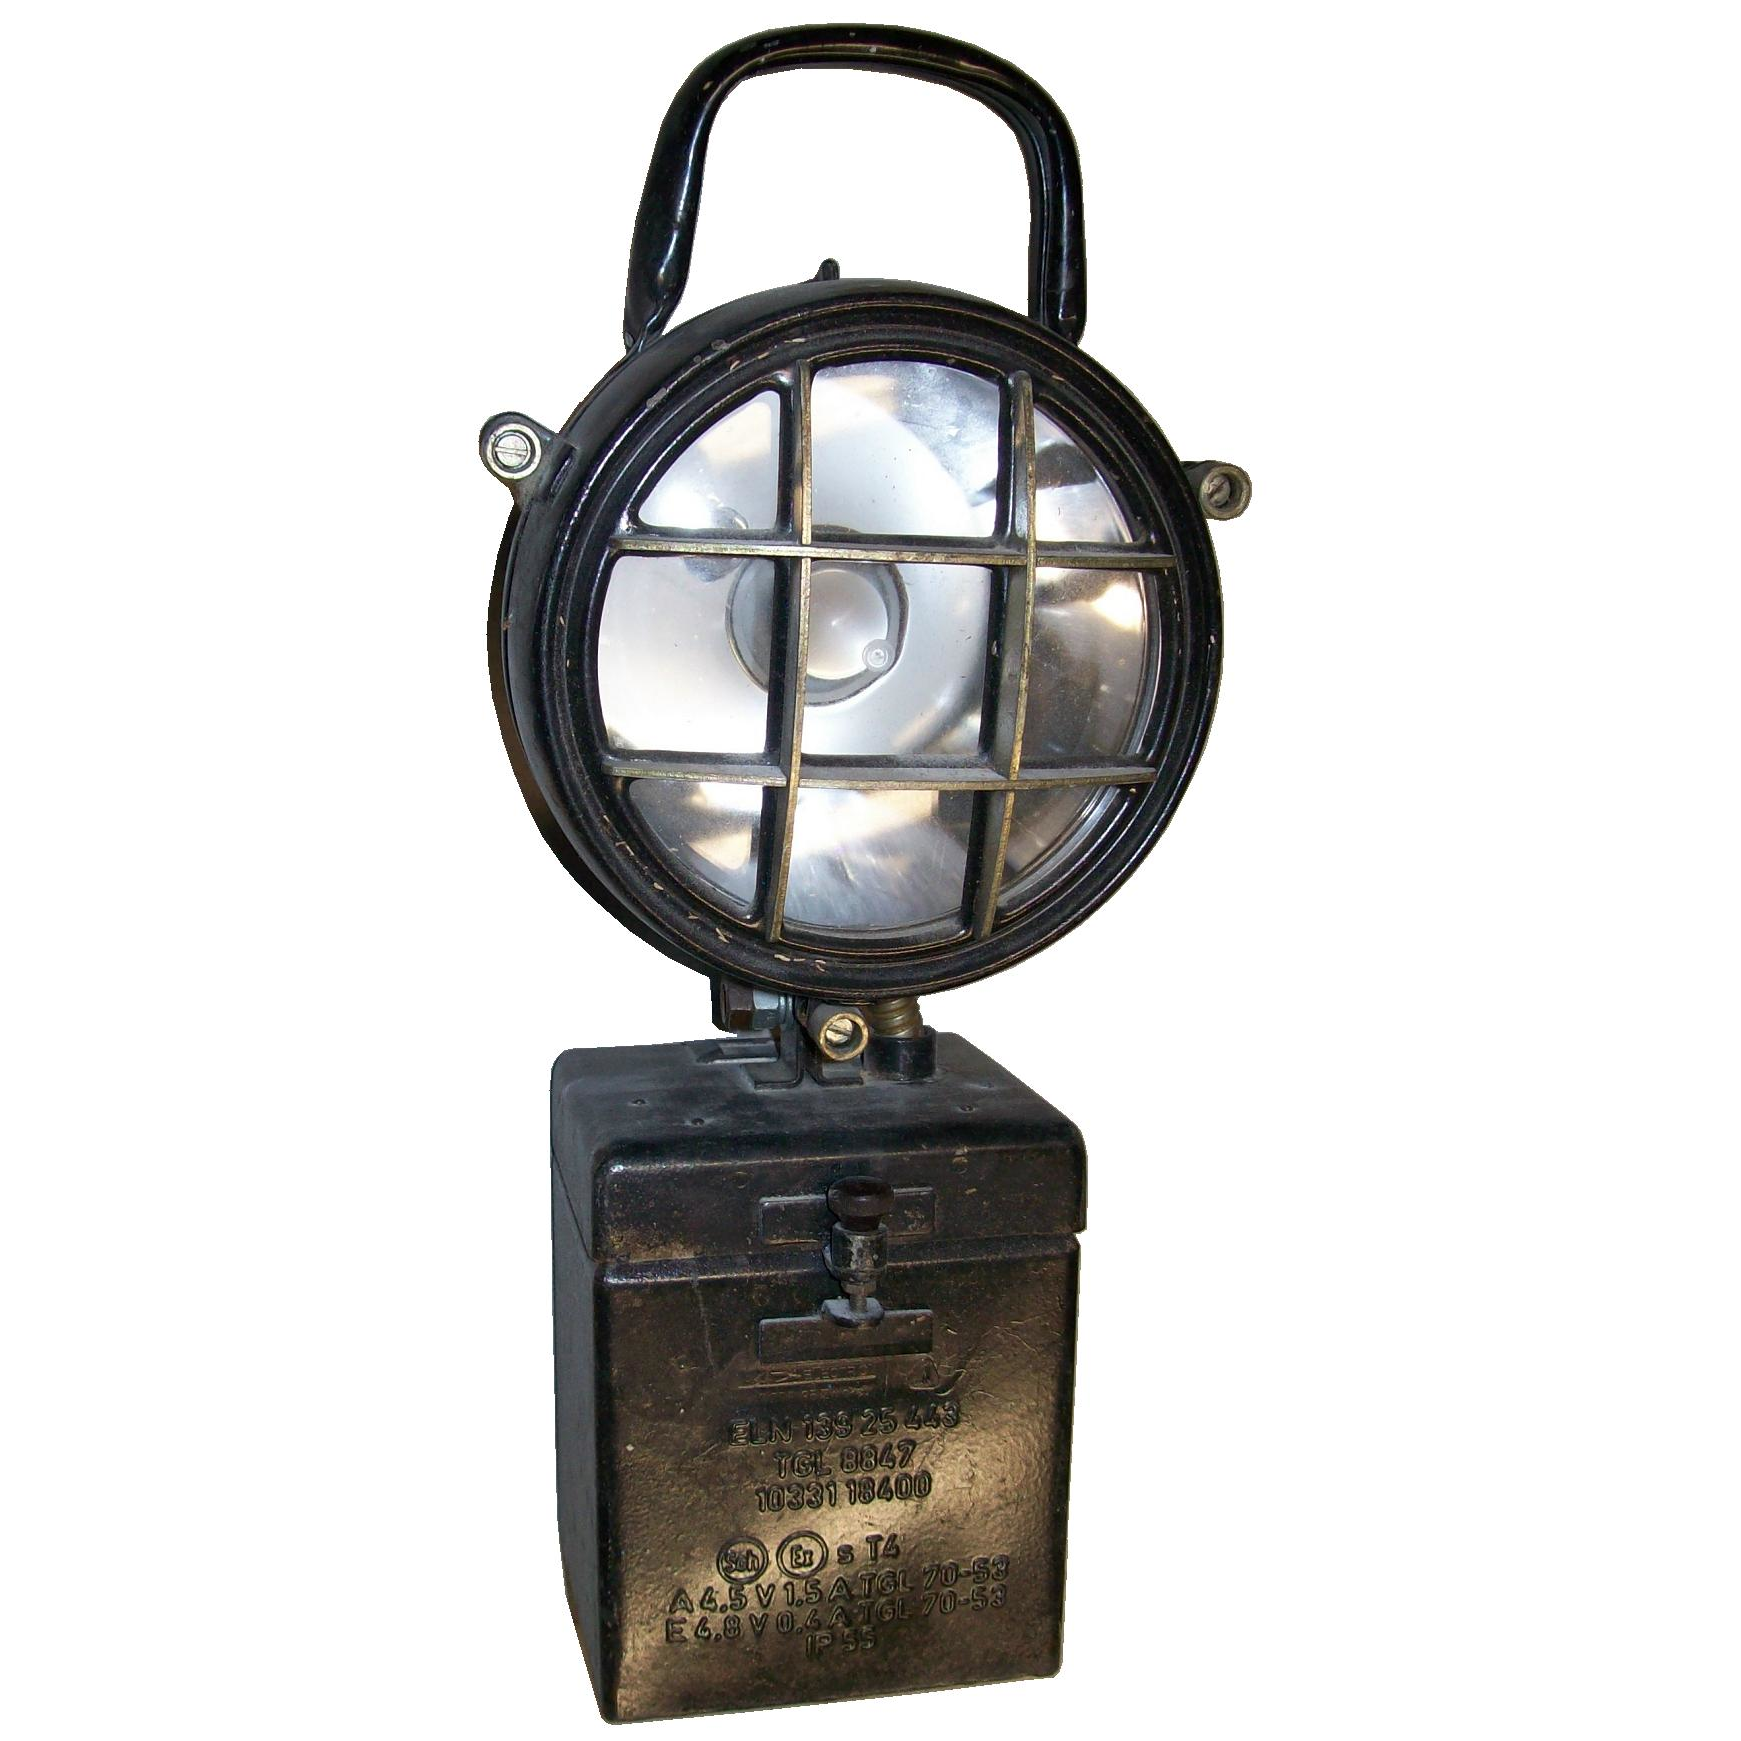
\includegraphics[width=\textwidth]{../SurvivalItemImages/minelamp}
        \end{minipage}\hfill
        \begin{minipage}{0.7\textwidth}
            \centering
            \Large Mine lamp
        \end{minipage}
    \end{figure}
    \vspace{-0.8em}
    \noindent\rule{\textwidth}{0.4pt}
            
    \begin{figure}[H]
        \centering
        \begin{minipage}{0.25\textwidth}
            \centering
            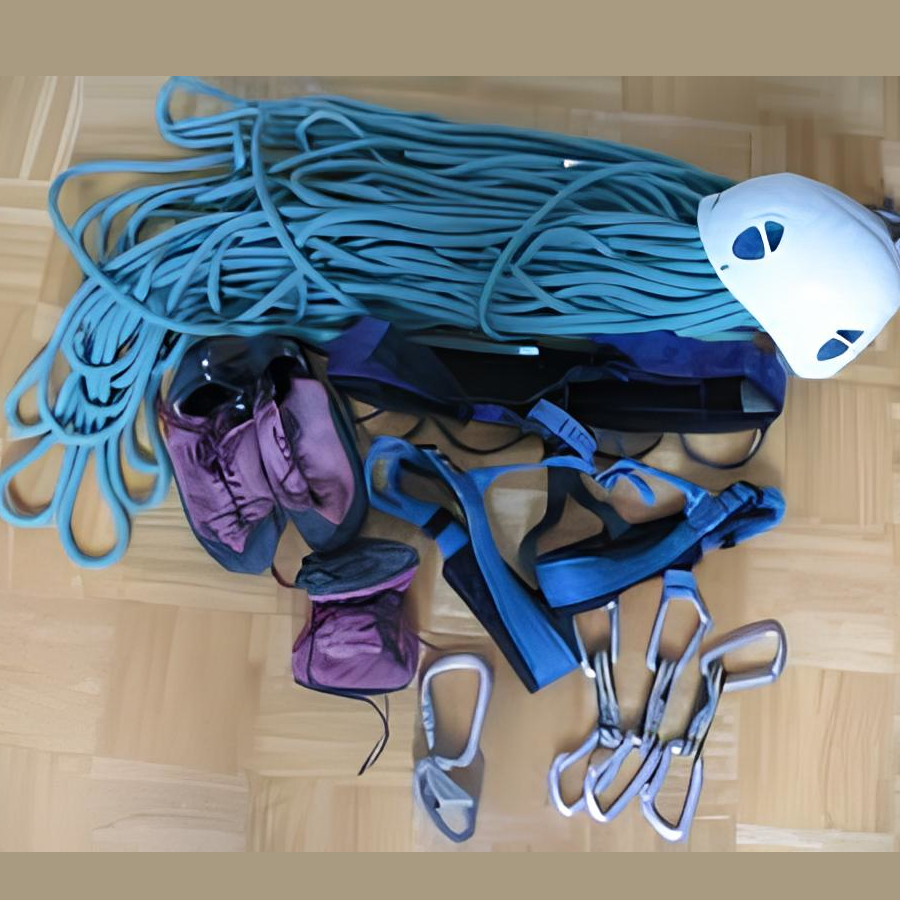
\includegraphics[width=\textwidth]{../SurvivalItemImages/climbinggear}
        \end{minipage}\hfill
        \begin{minipage}{0.7\textwidth}
            \centering
            \Large Climbing gear with reserve helmet
        \end{minipage}
    \end{figure}
    \vspace{-0.8em}
    \noindent\rule{\textwidth}{0.4pt}
            
    \begin{figure}[H]
        \centering
        \begin{minipage}{0.25\textwidth}
            \centering
            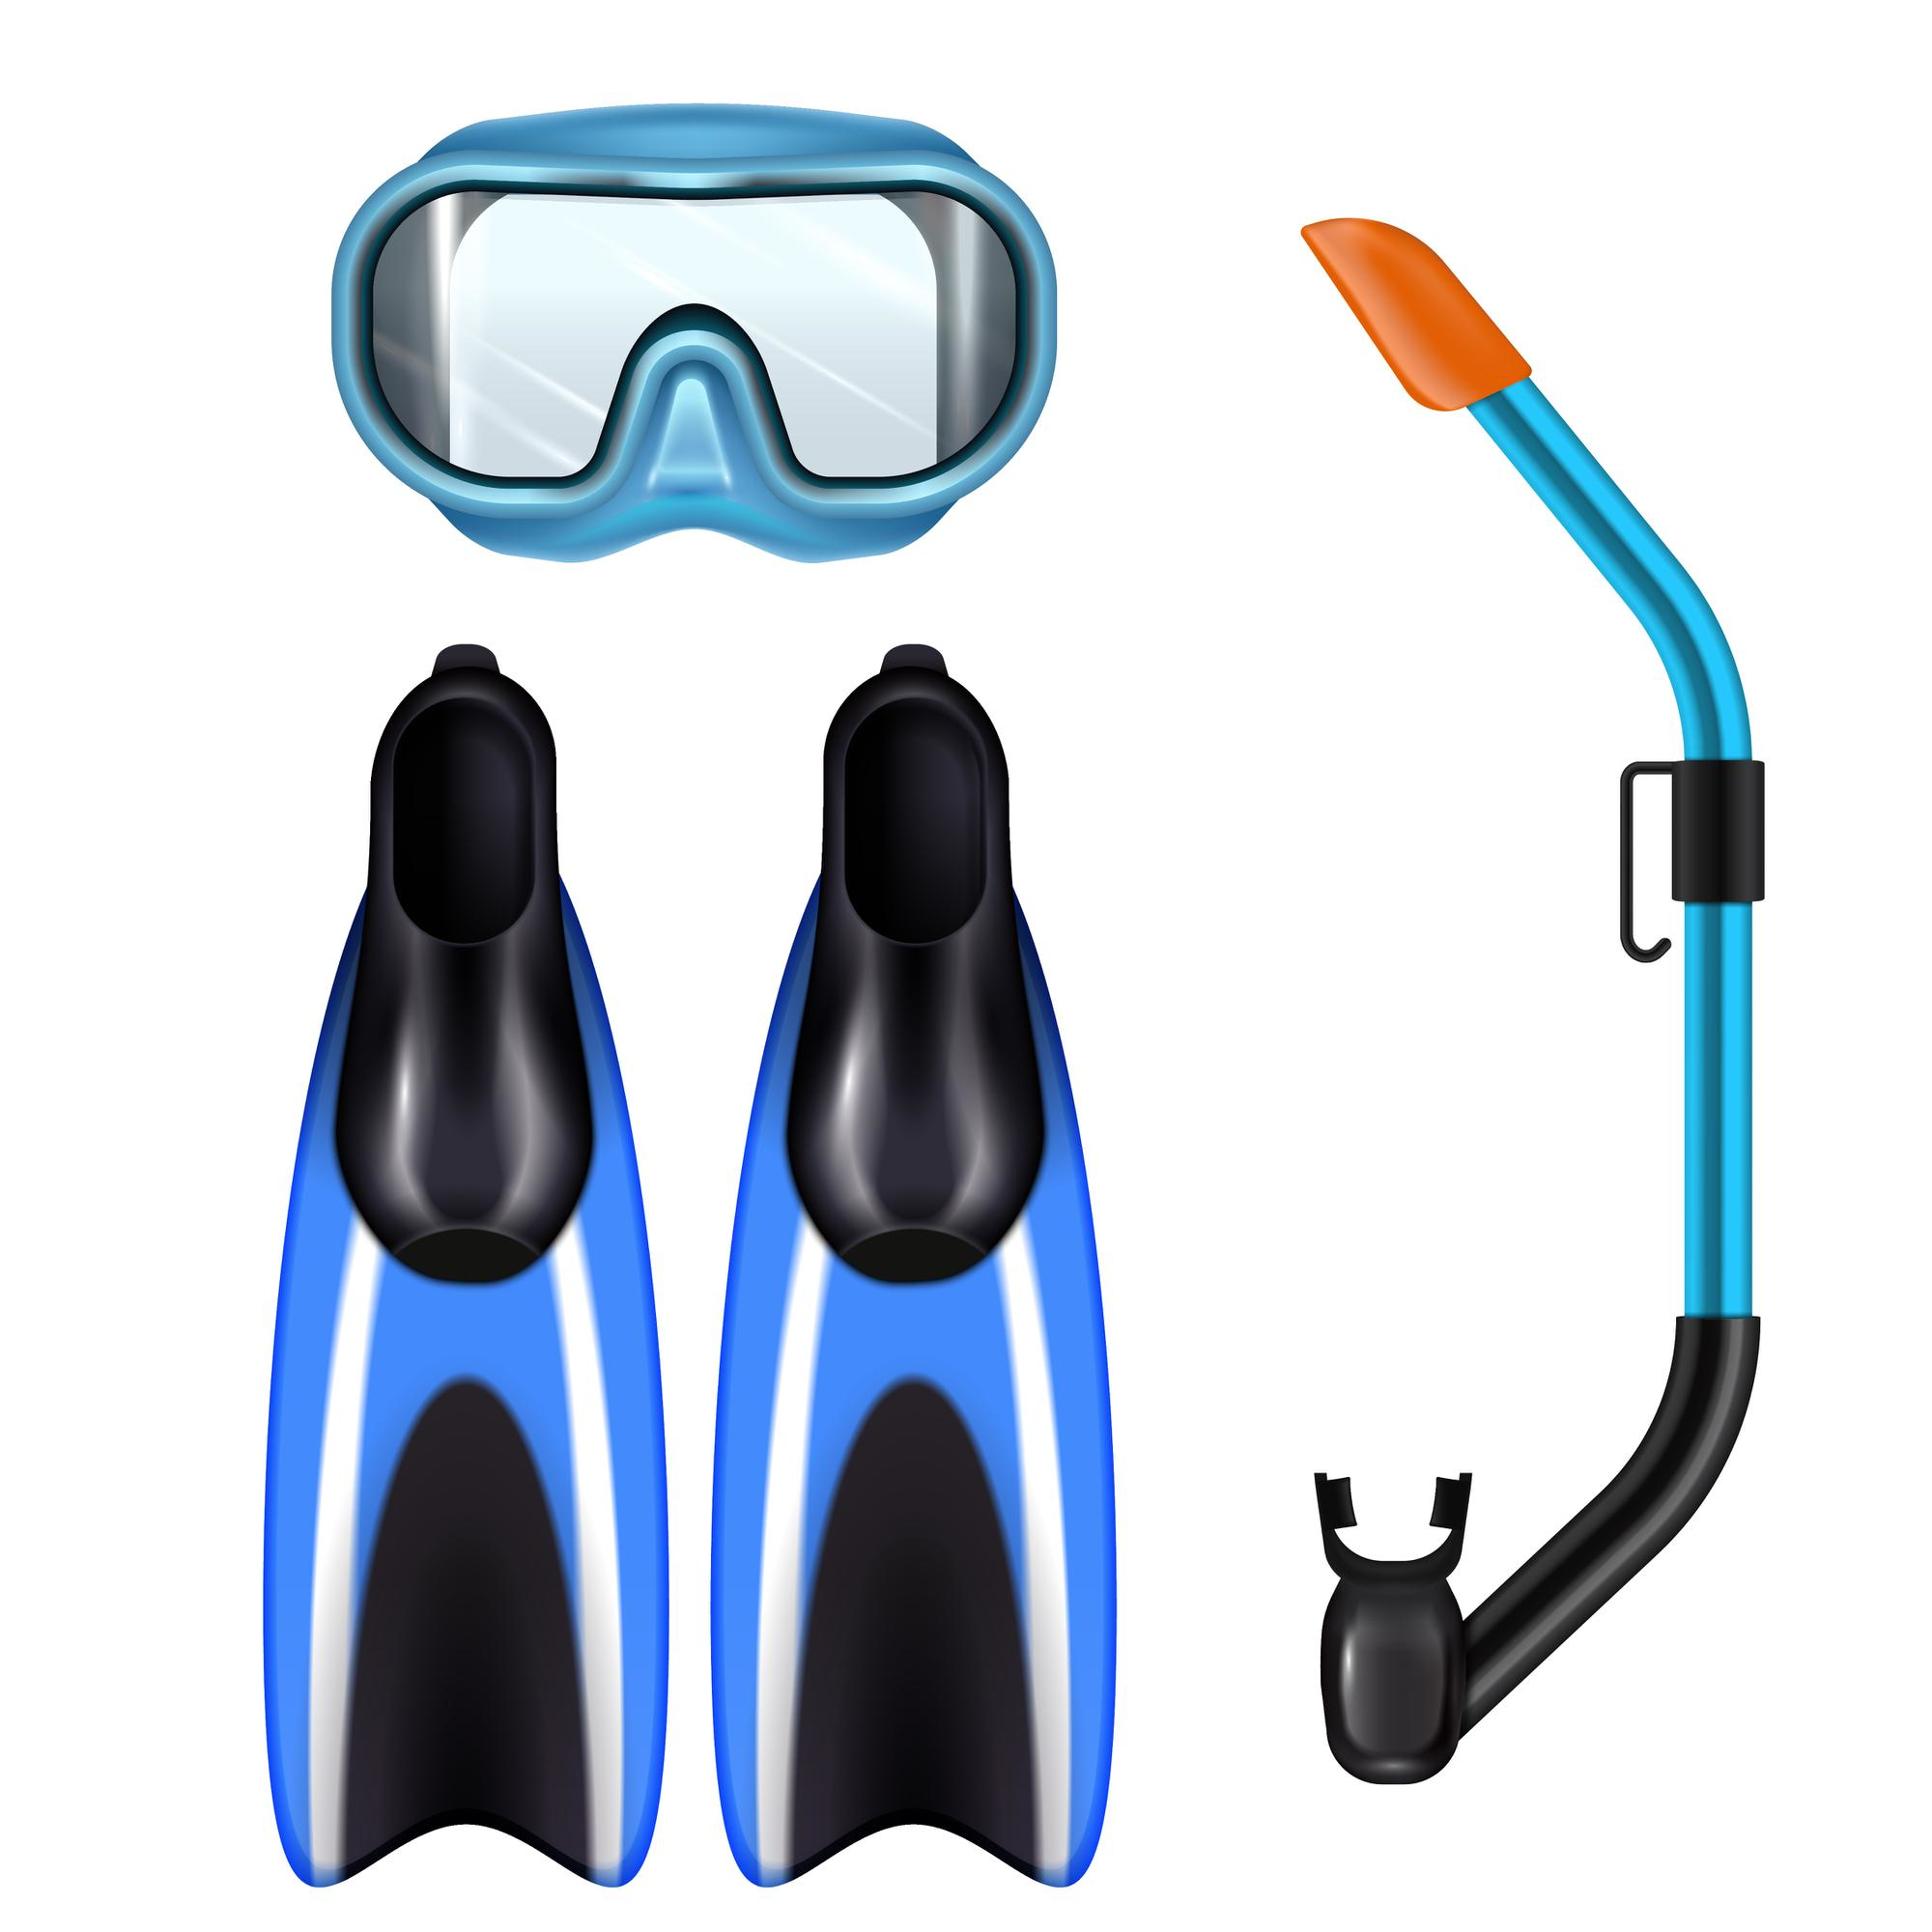
\includegraphics[width=\textwidth]{../SurvivalItemImages/divingequipment}
        \end{minipage}\hfill
        \begin{minipage}{0.7\textwidth}
            \centering
            \Large A simple diving equipment
        \end{minipage}
    \end{figure}
    \vspace{-0.8em}
    \noindent\rule{\textwidth}{0.4pt}
            
    \begin{figure}[H]
        \centering
        \begin{minipage}{0.25\textwidth}
            \centering
            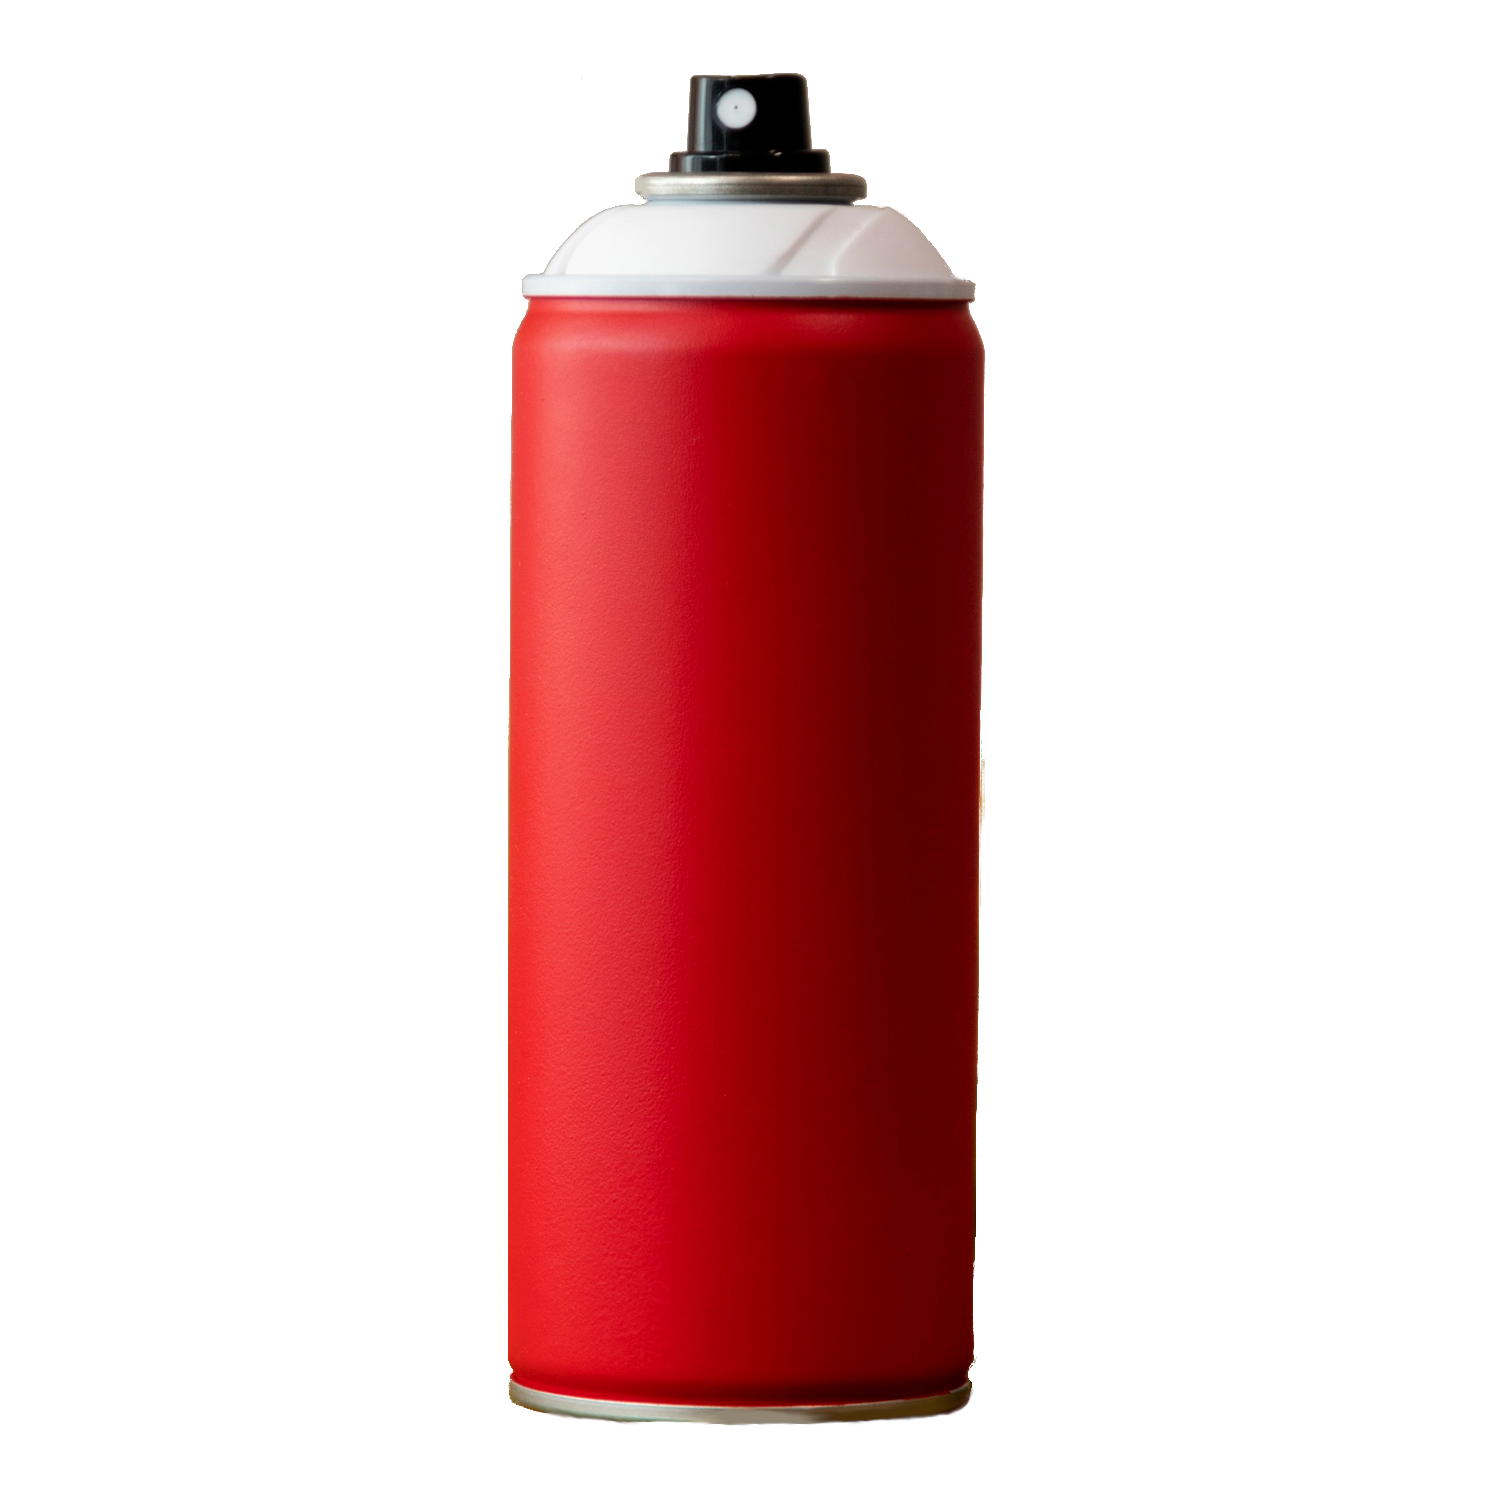
\includegraphics[width=\textwidth]{../SurvivalItemImages/spraycan}
        \end{minipage}\hfill
        \begin{minipage}{0.7\textwidth}
            \centering
            \Large Spray can with fluorescent paint
        \end{minipage}
    \end{figure}
    \vspace{-0.8em}
    \noindent\rule{\textwidth}{0.4pt}
            
    \clearpage
    \section*{Scenario: \textmd{Cavelabyrinth} \hfill Participant \textmd{2}}
    \Large You were on a tour through a large cave labyrinth with underground lakes for several days now. A tunnel crashed down, you and two fellow travelers were separated from the tour guide and the rest of the group. You also lost all possibilities to contact the others. Fortunately no one is injured and your protective clothes and helmet lamps are in good condition. The evening before, the tour guide explained that there are several exits from the cave, but it takes several days to reach those and one needs to cross some of the underground lakes. On your side of the collapsed tunnel you could find some items.\clearpage
        \end{document}
        